17. $(y-2x)\left(|x|-5-y
ight)=0\Leftrightarrow\left[\begin{array}{l}y-2x=0,\\ |x|=y+5.\end{array}
ight.\Leftrightarrow
\left[\begin{array}{l}y=2x,\\ \begin{cases}\left[\begin{array}{l}x=y+5,\\ x=-y-5.\end{array}
ight.\\ y+5\geqslant0\end{cases}\end{array}
ight.\Leftrightarrow
\left[\begin{array}{l}y=2x,\\ \begin{cases}\left[\begin{array}{l}y=x-5,\\ y=-x-5.\end{array}
ight.\\ y\geqslant-5\end{cases}\end{array}
ight.$
$$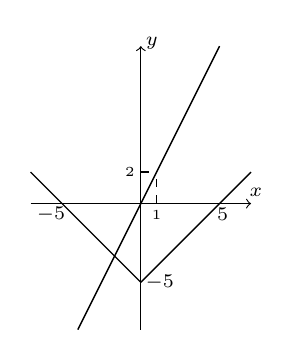
\begin{tikzpicture}[scale=0.2]
\tikzset {line01/.style={line width =0.5pt}}
\tikzset{line02/.style={line width =1pt}}
\tikzset{line03/.style={dashed,line width =0.5pt}}
%\filldraw [black] (0,0) circle (1pt);
\draw [->] (-7,0) -- (7,0);
\draw [->] (0,-8) -- (0,10);
\draw[line01] (-4,-8) -- (5,10);
\draw[line01] (7,2) -- (0,-5);
\draw[line01] (-7,2) -- (0,-5);
%\draw[line03] (-2,-1) -- (-2,1);
\draw[line03] (0,2) -- (1,2);
\draw[line03] (1,0) -- (1,2);
\draw (7.3,0.7) node {\scriptsize $x$};
\draw (1.2,-5) node {\scriptsize $-5$};
\draw (5.2,-0.7) node {\scriptsize $5$};
\draw (-5.7,-0.7) node {\scriptsize $-5$};
\draw (1,-0.7) node {\tiny $1$};
\draw (-0.7,2) node {\tiny $2$};
%\draw (-1.4,-0.5) node {\tiny $-2$};
%\draw (-3.5,-0.7) node {\tiny $-3$};
\draw (0.7,10.2) node {\scriptsize $y$};
%\draw (-2,-1) circle (8pt);
%\draw (-2,1) circle (8pt);
\end{tikzpicture}$$
